\documentclass[10pt,twocolumn,letterpaper]{article}

\usepackage{cvpr}
\usepackage{times}
\usepackage{epsfig}
\usepackage{graphicx}
\usepackage{amsmath}
\usepackage{amssymb}
\usepackage{csquotes}
\usepackage{float}
\usepackage{wrapfig}
\usepackage{bbm}

\DeclareMathOperator{\similar}{\mathrm{sim}}
% Include other packages here, before hyperref.

% If you comment hyperref and then uncomment it, you should delete
% egpaper.aux before re-running latex.  (Or just hit 'q' on the first latex
% run, let it finish, and you should be clear).
\usepackage[breaklinks=true,bookmarks=false]{hyperref}

\cvprfinalcopy % *** Uncomment this line for the final submission

\def\cvprPaperID{****} % *** Enter the CVPR Paper ID here
\def\httilde{\mbox{\tt\raisebox{-.5ex}{\symbol{126}}}}

% Pages are numbered in submission mode, and unnumbered in camera-ready
%\ifcvprfinal\pagestyle{empty}\fi
\setcounter{page}{4321}
\begin{document}
	
	%%%%%%%%% TITLE
	\title{Semi-Supervised Learning Task on Naver Fashion Dataset}
	
	\author{Junseok Choi(20190665)\\
		Team 7\\
		{\tt\small w\_choi@kaist.ac.kr}
		% For a paper whose authors are all at the same institution,
		% omit the following lines up until the closing ``}''.
		% Additional authors and addresses can be added with ``\and'',
		% just like the second author.
		% To save space, use either the email address or home page, not both
		\and
		Minyoung Hwang(20170738)\\
		Team 7\\
		{\tt\small myhwang99@kaist.ac.kr}
		\and
		Junghyun Lee(20170500)\\
		Team 7\\
		{\tt\small jh\_lee00@kaist.ac.kr}
	}
	
	\maketitle
	%\thispagestyle{empty}
	
	%%%%%%%%% ABSTRACT
	\begin{abstract}
		In this paper, we propose a novel semi-supervised learning(SSL) framework for CS492(I) Naver Fashion Dataset challenge. First, we propose a framework in which multiple SSL algorithms are combined in an orthogonal manner.
		Also, by analyzing the given training dataset and exploiting some common characteristics among the images, we propose using attention-based pre-training.
		Through extensive empirical studies, we show that our approach gives a high performance, placing $2$nd in the leaderboard.
	\end{abstract}
	
	%%%%%%%%% BODY TEXT
	\section{Introduction}
	{\it Semi-supervised learning (SSL)}, a learning framework where the training data is not labeled fully (usually, only a small percentage is labeled, and the rest is unlabeled), has received a lot of attention, lately.
	There has been two approaches to SSL methodology: regularization based method and pseudo-labeling based method.
	Regularization based method adds {\it unsupervised loss term} in order to account for the additional unlabeled data.
	Pseudo-labeling, first proposed in \cite{Lee13}, is a wrapper method in which unlabeled datas are given {\it pseudo labels}.
	
	As part of CS492(I), in this paper, we propose our solution to the SSL task with Naver Fashion Dataset.
	Unlike previous works, we propose a new framework in which various approaches are combined together to give better performance.
	(Specifically, the previously mentioned approaches fo SSL have been combined)
	
	Our contributions can be summarized as follows:
	\begin{itemize}
		\item We've achieved $2$nd place in CS492(I) leaderboard.
		
		\item By exploiting some of the common characteristics of the Naver Fashion Datset, we propose using attention as part of our SSL-based approach.
		
		\item We show empirically that as long as one considers methods that introduces improvements in non-overlapping way (i.e. \enquote{orthogonal}), then combining them leads to much better accuracy.
	\end{itemize}
	
	
	
	\section{Preliminaries}
	
	\subsection{Naver Fashion Dataset/Resources}
	Naver Fashion Dataset has $58735$ unlabeled images and $1060$ training labeled images.
	Due to the nature of our task, we weren't given any details of the test set.
	We note that even when compared to $1\%$ of the ImageNet ILSVRC-2012\cite{ILSVRC15}, the size of the given training data was too small.
	We also had some constraints on the amount of resources provided by NSML\cite{NSML}.
	
	
	\subsection{Assumptions}
	In this subsection, we discuss some common underlying assumptions in SSL.
	% , which can be summarized as follows: there is some informative correlation between the marginal distribution $p(x)$ and the posterior $p(y|x)$, where $x$ is a data and $y$ is a label.
	These assumptions are necessary in the sense that if they are not satisfied, then additional unlabeled data leads to degradation in performance, implying breakdown of the SSL framework.
	Some (but not many) previous works have dealt with such phenomenon. (As stated in \cite{Zhu05}, this can be attributed to \enquote{publication bias}.)
	For example, Cozman et al.\cite{CCC02} showed both theoretically and empirically that in some specific settings(mixture models) in which the assumptions do not hold, more unlabeled data may actually increase classification accuracy.
	(See also \cite{Elworthy94})
	
	First is the manifold assumption, which asserts that the data actually lies on a very low-dimensional manifold, submerged in $\mathbb{R}^d$.
	Second is the smoothness assumption, which asserts if $x, x' \in X$ are close together in $\mathcal{X}$, then the corresponding labels $y, y'$ should be the same.
	This is especially useful in SSL since if $x \in X_L$ and $x' \in X_U$ are close together, then there is a high probability (under this assumption) that $x'$ should be labeled with the same label as $x$, which is already known.
	Lastly, we have the low-density assumption, which asserts that the decision boundary of a classifier must pass through low-density regions in $\mathcal{X}$.
	A simple argument\cite{EH20} can be used to show that this assumption is actually a counterpart to the smoothness assumption.
	
	
	\section{Methodology}
	%In the following, we start with introducing the overall structure of our implementation, 
	Our approach consists of two part; representation learning and fine tuning.
	Let us explain each part in detail, then propose a method to combine all the mentioned algorithms.
	ALong with that, we discuss how our method achieves superior performance compared to prior works, focusing specifically on how our method is very suitable for Naver Fashion Data set.
	
	
	\subsection{SimCLR}
	First proposed in \cite{CKNH20}, SimCLR is a simple framework for constrastive learning of visual representations.
	Suppose that we have a minibatch of size $N$.
	
	A stochastic data augmentation: for each data $x$, two data transformations are performed to obtain $x_1, x_2$.
	These two are called to be a {\it positive pair} since they have to be similar.
	Rest of the pairs are said to be {\it negative}.
	A combination of random crop and color distortion was used.
	
	Constrastive loss function for a positive pair of samples is defined as follows:
	\[ l_{i,j} = -\log \frac{\exp\left(\similar(z_i, z_j) / \tau\right)}{\sum_{k=1}^{2N} \mathbbm{1}_{[k \not= i]} \exp\left( \similar(z_i, z_k) / \tau \right)} \]
	
	where $\similar(u, v) = \frac{u^\intercal v}{\lVert u \rVert \lVert v \rVert}$ is the cosine similarity.
	Using this loss, the base encoder $f(\cdot)$ and the projection head $g(\cdot)$ are updated.
	
	\subsection{Residual Attention Network}
	\begin{figure}
		\centering
		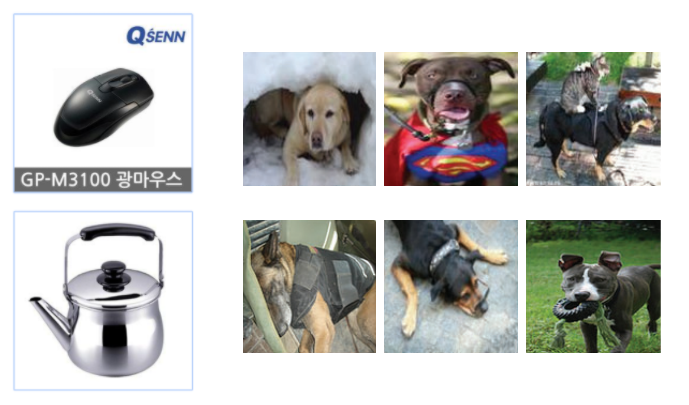
\includegraphics[width=7cm]{latex/naver_vs_imagenet.png}
		\label{fig:datasetcomparison}
		\caption{The leftmost two images are selected from the Naver Fashion Dataset and the other were chosen from ImageNet.}
	\end{figure}
	
	There is a clear distributive bias in Naver Fashion Dataset, which makes it very distinct compared to the commonly used datasets such as ImageNet(\cite{ILSVRC15}), as shown in Figure $1$. Since ImageNet samples are photos taken from the nature without any editing, the backgrounds are continuous and not separated from the object. However, images of our dataset are manually edited so that the objects are usually separated from other features like the captions and the removed backgrounds and then centered. The bias can be exploited to improve performance by choosing a model that better identify the more important areas of the given image. Residual Attention Network(\cite{RAN}) (RAN) creates an attention mask that ranges from 0 to 1 and element-wise multiply to the feature map to decide which part to pay more attention. The model then applies the mask on the previous feature map in a residual manner, so that the mask doesn't completely overwrite the useful features. This kind of ability makes it easier for the model to identify where the object is and pay less attention to the less important parts.\\
	
	\textbf{Optimization.} We modify the network to exploit the GPU resources we have as much as possible. The model parameters and forward passing uses half-precision float values instead of single-precision. This makes it possible to ramp up the pre-train batch size to about twice of the case without it. Due to compatibility issues, the batch normalization layers and the optimizer use single precision computation. As SimCLR is heavily dependent on batch size\cite{CKNH20}, we thought that it outweighed the precision decrease coming from using half-precision.
	
	% \begin{wrapfigure}
	% \includegraphics[width=\linewidth]{latex/navervsimagenet.png}
	% \label{fig:datasetcomparison}
	% \caption{Images selected from Naver Fashion Dataset and ImageNet. The leftmost two images are from the Naver Fashion Dataset and the other were chosen from ImageNet. }
	% \end{wrapfigure}
	
	
	
	\subsection{Consistency Regularization}
	
	Similarly to SimCLR, we applied the idea of smoothness assumption for finetuning. Unsupervised data augmentation \cite {Xie2020} is a method, where loss function consists of classification loss term over labeled data and consistency regularization term over unlabeled data. The brief flow of the work can be summarized as follows:
	\begin{itemize}
		\item For each given original input $x$, generate augmented pair $\bar{x}, \tilde{x}$.
		\item Predict distribution of labels for each augmented inputs $p_\theta\left(y|\bar{x}\right)$, $p_\theta\left(y|\tilde{x}\right)$ and optimize divergence $D\left(p_\theta\left(y|\bar{x}\right) \parallel p_\theta\left(y|\tilde{x}\right)\right)$.
	\end{itemize}
	In this work, we differed the strength of the augmentations, considering the low accuracy of the model's prediction. Each weak and strong augmentation produces $\bar{x}, \tilde{x}$, respectively. During back propagation, the $p_\theta\left(y|\tilde{x}\right)$ is enforced to mimic $p_\theta\left(y|\bar{x}\right)$. Formally, the consistency loss term is defined as following:
	\begin{equation}
		I\left(\max_y p_\theta\left(y|\bar{x}\right) > \beta\right) CE \left(p_\theta\left(y|\bar{x}\right)\parallel p_\theta\left(y|\tilde{x}\right)\right)
	\end{equation}
	
	As proposed in prior work \cite{Xie2020}, we added condition indicating confidence or reliability of the prediction. 
	
	\subsection{Label Propagation}
	
	Considering small number of labeled data set, the model may show too low accuracy to allocate pseudo-labels depending on itself. Instead, the model can learn good representation through unsupervised pre-task. It is reasonable to expect generating pseudo-labels based on inputs' representation vectors. The following explains a  label propagation method introduced from a prior work \cite{Iscen2019}.
	
	According to manifold assumption and smoothness assumption mentioned in \textbf{Section} 2, we can predict distribution of labels over entire data space using labeled data points as anchors. In detail, we introduce adjacency matrix $W$, which encodes relative position between each point, and defines pseudo-labels $Z$ of entire data as following:
	\begin{equation}
		Z=(I-\alpha W)^{-1}Y
	\end{equation}
	Here, $\alpha$ is an arbitrary weight and $Y$ is original labels, where labels for unlabeled data are initialized as $no label$ constant.
	
	Practical procedure consists of three steps. To begin with, we make a nearest neighbor graph and conduct label propagation. Next, we decide weight of each label considering the reliability of propagated distributions. The final step is performing the normal classification task using pseudo-labels for unlabeled data. Detailed steps are same as the prior work \cite{Iscen2019}.\\ 
	
	% \textbf{Nearest neighbor graph.} The model provides representation vector for each input. Then, \textit{affinity matrix} $A \in \mathbb{R}^{nxn}$ is defined as following:
	% \[a_{ij} = 
	%     \begin{cases}
	%         \left[ v_i^\intercal v_j \right]^\gamma, & \text{if } i \not= j, \ v_i \in NN_k(v_i) \\
	%         0 & \text{otherwise}
	%     \end{cases}
	% \]
	
	% where $NN_k(v)$ is the set of $k$ nearest neighbors of $v$.
	
	% Using $A$, adjacency matrix $W$ is calculated as $W := A + A^\top$.\\
	% \textbf{Label propagation.} 
	% Since direct calculation of $(I-\alpha W)^{-1}$ is complex, we use conjugate gradient (CG) method in order to find solution of linear system
	% $$ (I-\alpha W)Z = Y$$
	
	\subsection{Full Procedure.} To begin with, we train our self-attention model using SimCLR and move to finetuning. Model conducts classification task for finetuning. Finetuning procedure is divided into three sections. During the first section, model uses only labeled data. In the middle section, unlabeled data is inserted with pseudo labels resulted from label propagation. In last section, consistency regularization loss term is added with pairs of augmentation.\\
	\textbf{Advantages over previous approaches.} Our approach is a combination of well-known previous methods; label propagation \cite{Iscen2019} and consistency regularization \cite{Xie2020}. There are problems in using each one alone. In trivial, consistency regularization works well after model's accuracy increases to some extent. Label propagation seems to be direct solution for the problem, but it is easy to converge to trivial solution, since augmentation on inputs for classification is weak. We expect that addition of consistency term may help the model to conduct classification task referring to general feature of inputs and escape such regions. We confirmed our belief through ablation test in \textbf{Section} 4.
	
	\section{Experiments}
	% \cite{EH20} observes that the choice of data sets and their partitioning have a significant impact on the relative performance of different learning algorithms
	% In the case of SSL, some critical choices include amount of labeled datas, baseline model.
	% This work won't be considering a diverse range of datasets, because the only dataset available for use was the Naver Fashion Datset, whose training-test split was also beyond our control.
	All of our codes have been made publicly available in Github repository\footnote{\url{https://github.com/cs492i-ELSA/cs492i_cv_repo_7}}.
	
	\subsection{Effects of various components}
	\subsubsection{Self-Attention}
	\begin{figure}
		\centering
		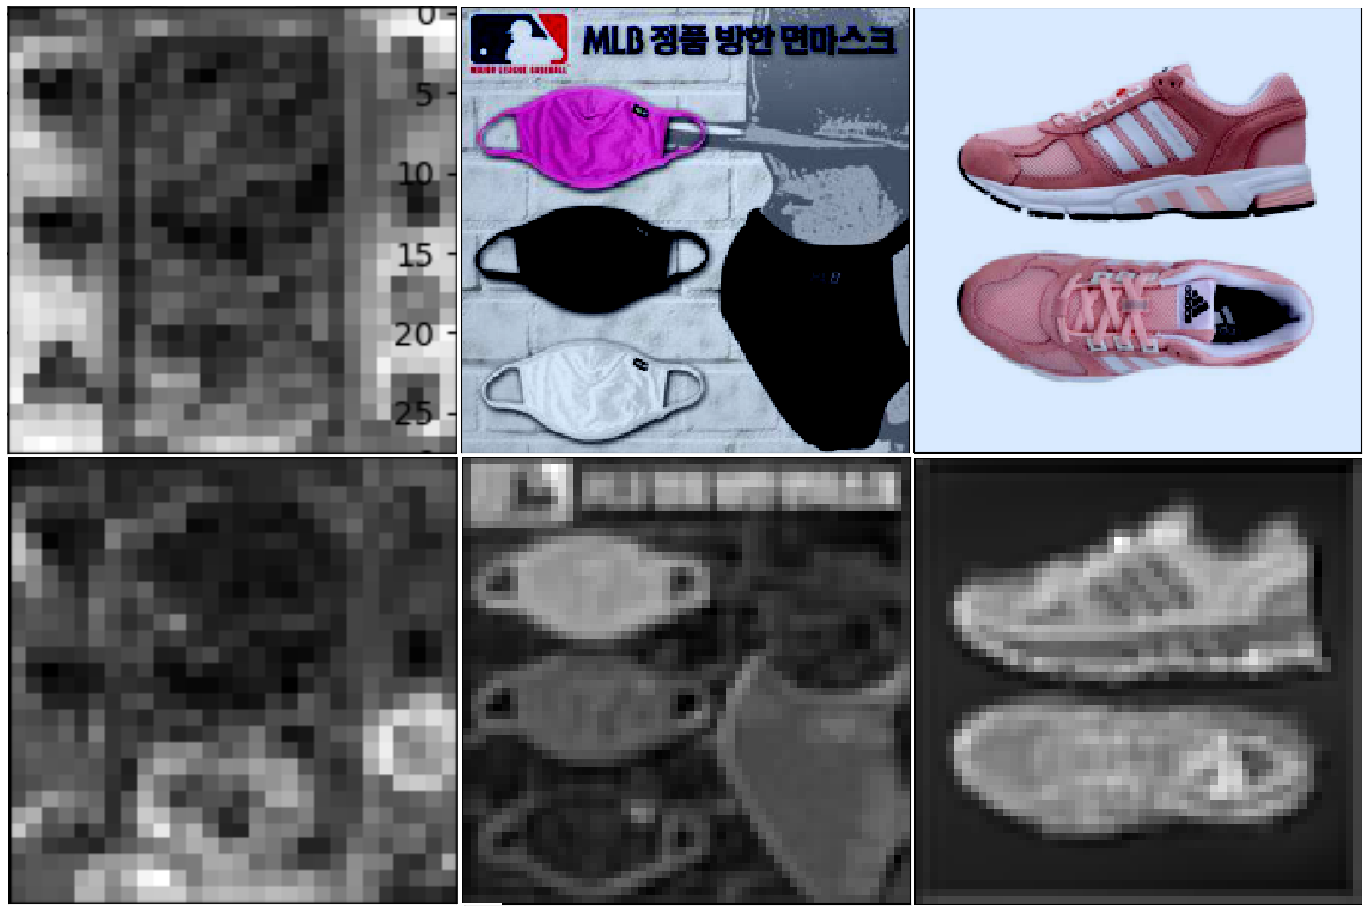
\includegraphics[width=6cm]{latex/features.png}
		\label{fig:features}
		\caption{Starting from the top left image, in clockwise: 1) a feature map before attention layer, 2) an input mask image, 3) an input shoe image, 4) a shoe image feature map after an attention layer, 5) a mask image feature map after an attention layer, 6) a feature map after attention layer.}
	\end{figure}
	\begin{table}
		\centering
		\label{table:RANvsResNet}
		\begin{tabular}{ ||p{1.45cm}|c c||  }
			\hline
			Model & Top 1 Acc. (\%) & Top 5 Acc. (\%)\\
			\hline
			ResNet50&  0.083 & 0.208  \\
			RAN56&  0.423 & 0.226  \\
			ResNet101&  0.045 & 0.087  \\
			RAN92&  0.426 & 0.215  \\
			\hline
		\end{tabular} \\ [1ex]
		\caption{Comparison of test set accuracy before label propagation using the best of each model.}
	\end{table}
	Since self-attention layer is simply added on top of the ResNet architecture, it was possible to compare the performances where attention was used and where not. We believe the attention layer of our model is improving ResNet, which we verify quantitatively and qualitatively.\\\\ \textbf{Quantitative Analysis.} RAN architecture has the best test accuracy, and it seems that the additional attention layer enables the model to handle large number of parameters more efficiently, since simply using larger ResNet model with SimCLR didn't result in a good accuracy. We hypothesize that this is due to the negative effects of small batch size on SimCLR (180 for ResNet101), where we're forced to use when using a large model. \\\\
	\textbf{Qualitative Analysis.} We examined the intermediate layer output of our model. From 1) and 6) of Figure $2$ we can observe our model erasing the less important parts of feature maps where the object is at the middle and there are colored captions at both sides. In 2), 5) and 3), 4), the model focuses more on the objects and ignore the background, including its patterns. 
	
	
	
	\subsubsection{Orthogonal combination of methods}
	This is shown through a series of experiments in which an incremental increase in performance is observed by adding on each method. The followings are details of our experiments, beginning with experiments applying consistency regularization and label propagation each alone, and our final proposal, combination of them.\\
	\textbf{Consistency regularization.} The training is performed for 20 epochs in total. Entire labeled and unlabeled data set is used as training set throughout the training.  The loss term consists of classification loss for labeled data and consistency regularization term for unlabeled one. Random resized cropping to size $224\times224$ followed by random horizontal flipping is applied in common. The difference is addition of color distortion between them for strong augmentation. A batch consists of two sub-batches for 64 labeled and 64x30 unlabeled inputs. The initial learning rate $l_0$ is 0.02 and decays by 0.1 for every 6 epochs.\\
	\textbf{Label propagation.} Whole procedure is divided into 2 stages. In first stage, classification task is conducted only for labeled data. This stage is up to 20 epochs. Before moving on to second stage, label propagation occurs and pseudo-labels are allocated to entire data including unlabeled ones. In second stage, model is trained by classification task over complete data set. Only weak augmentation in previous experiment is used. Batch consists of 2 labeled data and 32 unlabeled data. Learning rate maintained as 0.02 for 10 epochs and them decayed to 0.002 for left 14 epochs.\\
	\textbf{Consistency preserving label propagation.} The brief procedure is introduced in \textbf{Section} 3. Hyper parameters are same as ones in previous experiment using label propagation. The one difference is that consistency regularization loss term is added to original classification loss since 10 epochs after label propagation. The term is for both labeled and unlabeled data.\\
	\textbf{Performance of each approaches.} Figure \ref{fig:CRvsLPcomparison} shows the progress of top-1 accuracy of training using consistency regularization and label propagation each alone. One using consistency regularization quickly converges to about 20\%, which is easily achieved by using only labeled data. As we expected, label propagation have showed much better performance. Interestingly, Figure \ref{fig:LPvsLP+CRcomparison} and Table \ref{table:CRvsLPvsLPCR} proves that its performance gets even better after addition of consistency regularization.
	
	
	\begin{figure}
		\centering
		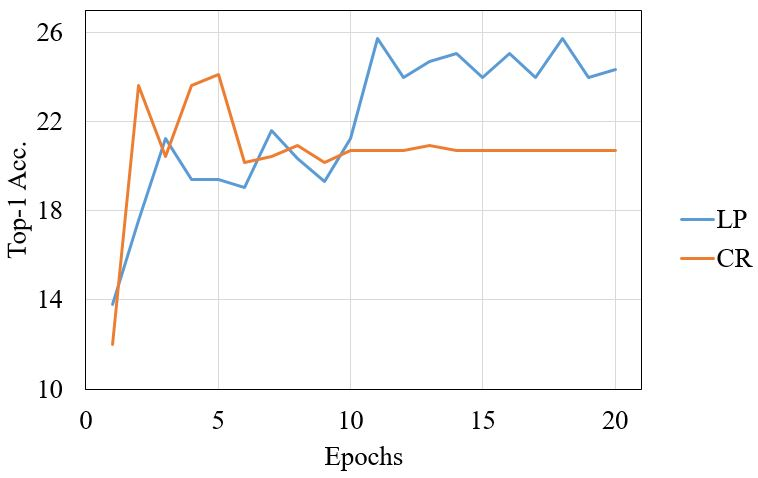
\includegraphics[width=7cm]{CRvsLP.JPG}
		\label{fig:CRvsLPcomparison}
		\caption{Accuracy of two models trained using consistency regularization and label propagation, respectively.}
	\end{figure}
	
	\begin{figure}
		\centering
		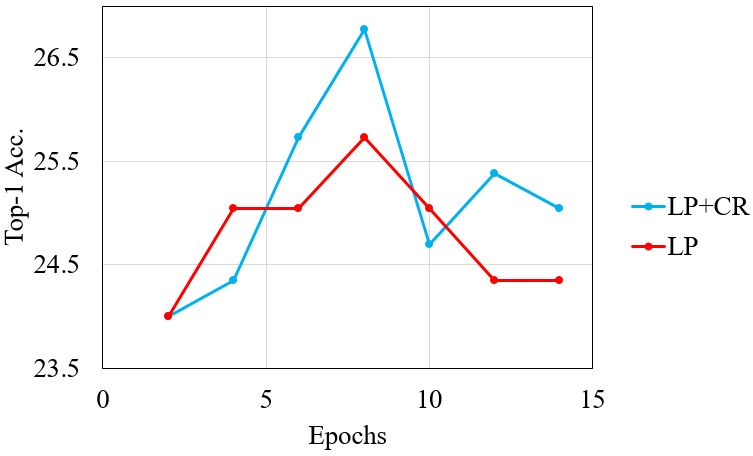
\includegraphics[width=7cm]{LPvsLP+CR.JPG}
		\label{fig:LPvsLP+CRcomparison}
		\caption{Accuracy of model after addition of consistency loss against pure one using only label propagation.}
	\end{figure}
	
	% Replaced with a Table
	%\begin{figure}
	%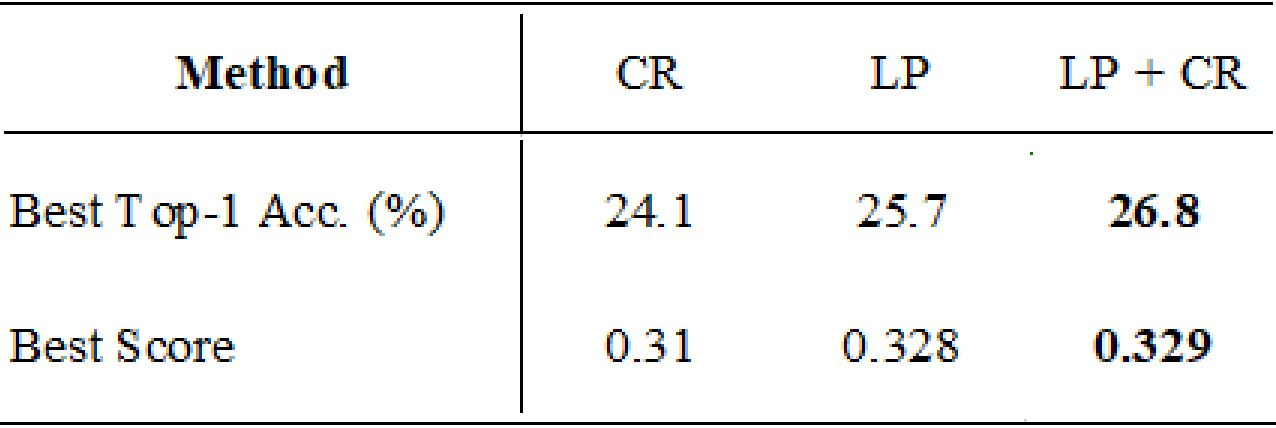
\includegraphics[width=\linewidth]{latex/ScoreTable.JPG}
	%\label{fig:datasetcomparison}
	%\caption{The leftmost two images are selected from the Naver Fashion Dataset and the other were %chosen from ImageNet.}
	%\end{figure}
	
	\begin{table}
		\centering
		\label{table:CRvsLPvsLPCR}
		\begin{tabular}{ p{1.5cm}|c c  }
			Method & Best Top-1 Acc. & Best Score\\
			\hline
			CR & 24.1 & 0.310  \\
			LP & 25.7 & 0.328 \\
			LP + CR & \textbf{26.8} & \textbf{0.329} \\
			\hline
		\end{tabular} \\ [1ex]
		\caption{Comparison of three approaches.}
	\end{table}
	
	
	\subsubsection{Hyperparameter Tuning}
	We performed a learning rate sweep in $\{0.0005, 0.001, 0.002, 0.005, 0.01\}$ and selected the best optimizer among SGD, SGD+LARS(\cite{LARS, torchLARS}), Adam(\cite{Adam}) and Yogi(\cite{Yogi}). We also used both Exponential and Multi-step scheduler provided by PyTorch. Finally, we always used the largest batch possible for pre-training which was not big enough to add instability to the training and did a batch size sweep on the fine-tuning process, where we freeze the pre-trained model. Our best result was achieved using Adam, exponential scheduler and fine-tuning batch size 512. The performance degraded after size of 512, which we hypothesize is because of the large batch size and a lack of efficiency of the LARS optimizer when the pretrained model frozen and not updated.
	
	
	\section{Conclusion}
	In this work, we present a new approach to SSL by combining orthogonal procedures.
	We use an attention-based model that can efficiently exploit the dataset-specific characteristics. Then SimCLR was used for pre-traning, and UDA and label propagation for fine-tuning, followed by hyperparameter tuning. We also perform an ablation study and verify our method makes a significant improvement over the baseline. By using our framework, we achieved $2$nd place in the leaderboard.
	% This suggests that even though there are a lot of works that proposes new frameworks, combining existing frameworks together is also a promising avenue.
	% possible victim: and verify our method makes a significant improvement over the baseline.
	
	{\small
		\bibliographystyle{ieee_fullname}
		\bibliography{egbib}
	}
	
\end{document}
